\chapter{Strong fluctuation theorem for environmental entropy}
\label{chap:thingie}

The contents of this chapter were published in Physical Review E, ``Strong fluctuation theorem for nonstationary nonequilibrium systems'' \cite{thingie-paper}. The following is an elaborate description of its contents.

This chapter has two main parts. The first one provides an introduction to fluctuation theorems, Markov processes, entropy, and the terminology used. The secone one then uses these definitions to prove a new general fluctuation theorem, specializes it to appear in a more familiar form, and finally puts it to the test in two numerical examples.


%%%%%%%%%%%%%%%%%%%%%%%%%%%%%%%%%%%%%%%%%%%%%%%%%%%%%%%%%%%%%%%%%%%%%%%%%%%%%%
\section{Preliminaries}
%%%%%%%%%%%%%%%%%%%%%%%%%%%%%%%%%%%%%%%%%%%%%%%%%%%%%%%%%%%%%%%%%%%%%%%%%%%%%%



%%%%%%%%%%%%%%%%%%%%%%%%%%%%%%%%%%%%%%%%%%%%%%%%%%%%%%%%%%%%%%%%%%%%%%%%%%%%%%
\subsection{Fluctuation theorems}
%%%%%%%%%%%%%%%%%%%%%%%%%%%%%%%%%%%%%%%%%%%%%%%%%%%%%%%%%%%%%%%%%%%%%%%%%%%%%%

Classical thermodynamics is a theory of averages of certain quantities. For example, temperature is a measure for the \emph{mean} energy per degree of freedom of a gas, or the \emph{mean} cost of energy to increase the \emph{mean} entropy by a certain amount. Unfortunately, this approach requires certain quantities to exist a priori, and does not explain their origins. On the other hand, statistical physics typically starts with all individual constituents at the same time, and tries to explain how certain statistical properties -- the mean being just one of them -- emerge. In that sense, fluctuation theorems are about \textbf{taking away the averages} of classical thermodynamics. One of these averages is the entropy of a system \TODO{ref zum Vorspann}, of which we know that it obeys the second law of thermodynamics, typically written as
%
\begin{equation}
	\label{eqn:2nd_law_classical}
	\d S \geq 0 ~,
\end{equation}
%
meaning that thermodynamic (macroscopic) entropy is always increasing.

However, looking at the microscopic properties of a system, it is indeed possible that entropy spontaneously decreases -- when all microstates occur with some nonzero probability, there is also always a nonzero (albeit small) chance of transition to a highly ordered system. Fluctuation theorems provide a characteristic expression for the likelihood for certain statistical events to occur in a system. For example in the case of microscopic total entropy changes \(\Delta S\), it can be shown that
%
\begin{equation}
	P(\Delta S) = e^{\Delta S}P(-\Delta S)
\end{equation}
%
which states that the probability of spontaneous entropy increase by \(\Delta S\) is exponentially more likely than a decrease by the same amount; theorems of the above form will be referred to as \textbf{detailed} fluctuation theorems, as the expression yields symmetry information for each point of a distribution individually. In a sense, this is the analogon to the Second~Law from the viewpoint of statistical physics, and indeed it can be shown that \RefEqn{eqn:2nd_law_classical} can be recovered from this formula: integrating both sides yields
%
\begin{equation}
	\label{eqn:average of exp}
	1 = \inflint \d (\Delta S) P(\Delta S) = \inflint \d (\Delta S) e^{\Delta S}P(-\Delta S) = \left\langle e^{-\Delta S} \right\rangle
\end{equation}
%
which, using Jensen's inequality \(\langle e^x\rangle \geq e^{\langle x\rangle}\), implies
%
\begin{equation}
	\langle\Delta S\rangle \geq 0 ~.
\end{equation}
%
Averages of this form are known as \textbf{integral} fluctuation theorems.

It turns out that this derivation was overly general: in fact, a detailed fluctuation theorem implies arbitrarily many integral fluctuation theorems, since
%
\begin{align}
	   B
	&\equiv \langle e^{-\frac x2}A(x)\rangle
	= \inflint\d x \, P(x) e^{-\frac x2}A(x)
	= \int\limits_\infty^{-\infty}\d(-x) P(-x) e^{\frac x2}A(-x) \notag \\
	&= - \inflint\d x \, P(x) e^{-\frac x2}A(x)
	 = -B
	 = 0 \notag \\
	\label{eqn:antisymmetric exp average}
	&\Rightarrow
	\langle e^{-\frac x2}A(x)\rangle = 0
\end{align}

%
where \(A\) is an arbitrary antisymmetric function; the relation \RefEqn{eqn:average of exp} can be recovered by setting \(A(x) = \sinh(x/2) = \frac12(e^x-e^{-x})\).

This was but one example of a fluctuation theorem for \(\Delta S\); there are many more for other quantities (such as different forms of heat, work, other sub-categories of entropy), as can be seen e.g. in \cite{seifert-review}, and one of the main results of this chapter will be yet another entire class of fluctuation theorems.


%%%%%%%%%%%%%%%%%%%%%%%%%%%%%%%%%%%%%%%%%%%%%%%%%%%%%%%%%%%%%%%%%%%%%%%%%%%%%%
\subsection{Markov jumping processes}
\label{sec:markov process}
%%%%%%%%%%%%%%%%%%%%%%%%%%%%%%%%%%%%%%%%%%%%%%%%%%%%%%%%%%%%%%%%%%%%%%%%%%%%%%

A \emph{jumping process} is a system consisting of a discrete number of states that, governed by certain transition rates or probabilities, switches from one state to another repeatedly. A \emph{Markov process} is a special jumping process where the ``next'' state can only depend on the current state, and has no knowledge about its history. In other words, a Markov process is one in which the system does not have a concept of ``momentum'' in the colloquial sense.

An example for a jumping process is a gambler in a casino, the state being how much money he has. Each time he places a bet, he changes his state (loses or wins money).
%
\begin{enumerate}
	\item A realistic gambler can be seen jumping process, and can make his bets dependent on e.g. whether he lost his last game (which requires to know about the current balance and the one before that), or if he is suspicious kind could alter the winning probabilities in his favour. Note that the concept of ``winning streaks'' also falls into this category, as ``having'' one requires knowledge of the previous games/balances.
	\item A Markovian gambler would decide how much to bet based solely on how much money he currently has (and possibly how late it is). He would base none of his decisions on his knowledge about previous games.
\end{enumerate}






%%%%%%%%%%%%%%%%%%%%%%%%%%%%%%%%%%%%%%%%%%%%%%%%%%%%%%%%%%%%%%%%%%%%%%%%%%%%%%
\subsection{Terminology}
%%%%%%%%%%%%%%%%%%%%%%%%%%%%%%%%%%%%%%%%%%%%%%%%%%%%%%%%%%%%%%%%%%%%%%%%%%%%%%

Suppose we have a system \(\Omega\) of \(N\) states, enumerated by \(j\). Time runs from \(t = 0\) to \(t = T\). At times \(\tau_j\), the system transitions from an old state \(n_{j-1}\) into a new one. \(c_j\). Grouping multiple successive state changes together, we can describe the history of the system using a trajectory through time/state space with \(J\) jumps,
%
\begin{align}
	\gamma &=~
	\newcommand\iarrow[1]{~\underset{\tau_{#1}}\longrightarrow~}
	%
	c_0
	\iarrow{1}
	c_1
	\iarrow{2}
	\cdots
	\iarrow{j}
	c_{j}
	\iarrow{j+1}
	c_{j+1}
	\iarrow{j+2}
	\cdots
	\iarrow{J}
	c_{J}
	\\
	&= \{c_{i,\tau_i}\}
\end{align}
%
An ``element'' \(c_{i,\tau_i}\) of \(\gamma\) can thus be interpreted as ``the system is in state \(c_i\) starting at time \(\tau_{i}\), until \(\tau_{i+1}\)''. A visualization of the above description can be found in \RefFigure{fig:discrete_jumping_process}.

\begin{figure}[htb]
	\centering
	\begin{tikzpicture}
	[>=stealth]

	% coordinate system
	\begin{scope}
		% axes
		\begin{scope}[->]
			\newcommand\Excess{0.2}
			\draw (-\Excess,0) -- (10.5,0); % x
			\draw (0,-\Excess) -- (0,6);  % y
		\end{scope}


		\newcommand{\TickLength}{0.2}
		\newcommand{\LabelOffset}{0.5}
		
		% y axis labels/ticks
		\begin{scope}
			\foreach \y in {1,...,5} {
				\draw (-\TickLength/2, \y) -- (\TickLength/2, \y);
 				\node at (-\LabelOffset, \y) {\(\y\)};
			}
			\node at (0, 6 + \LabelOffset) {\(\Omega\)};
		\end{scope}

		% x axis labels/ticks
		\begin{scope}
			\foreach \i/\x in {0/0, 1/2, 2/3, 3/6, 4/7.5, 5/8, 6/10} {
				\draw (\x, -\TickLength/2) -- (\x, \TickLength/2);
				\node at (\x, -\LabelOffset) {\(\tau_\i\)};
			}
			\node at (0, -2*\LabelOffset) {\(0\)};
			\node at (10, -2*\LabelOffset) {\(T = \tau_{J+1}\)};

			\node at (10.5 + \LabelOffset, 0) {\(t\)};
		\end{scope}

	\end{scope}

	% Path taken
	\begin{scope}
		
		% Actual path
		\begin{scope} [thick]
			\draw (0,1) -- (2,1)
				(2,4) -- (3,4)
				(3,3) -- (6,3)
				(6,5) -- (7.5,5)
				(7.5,1) -- (8,1)
				(8,2) -- (10,2)
				;
			\newcommand{\Radius}{0.03}
			\foreach \xy in {(0,1), (2,1), (2,4), (3,4), (3,3), (6,3), (6,5), (7.5,5), (7.5,1), (8,1), (8,2), (10,2)} {
				\draw[fill=black] \xy circle (\Radius);
			}
		\end{scope}

		% Connecting jump lines
		\begin{scope} [dotted]
			\draw (2,1)-- (2,4)
			      (3,4) -- (3,3) 
				(6,3) -- (6,5) 
				(7.5,5) -- (7.5,1) 
				(8,1) -- (8,2)
				;
		\end{scope}

		% labels
		\begin{scope}
			\newcommand{\LabelOffset}{0.5}
			\node at (1,         1 - 0.5*\LabelOffset) {\small \(c_0 = 1\)};
			\node at (2.5,       4 + 0.5*\LabelOffset) {\small \(c_1 = 4\)};
			\node at (4.5,       3 - 0.5*\LabelOffset) {\small \(c_2 = 3\)};
			\node at (6.75,      5 + 0.5*\LabelOffset) {\small \(c_3 = 5\)};
			\node at (7.75,      1 - 0.5*\LabelOffset) {\small \(c_4 = 1\)};
			\node at (9,         2 + 0.5*\LabelOffset) {\small \(c_5 = 2\)};
		\end{scope}

		% final dashed line at t=T

		\begin{scope}
			\draw [dashed] (10,0) -- (10,6);
		\end{scope}
		
	\end{scope}

\end{tikzpicture}

	\caption[]{Visualization of a discrete jumping process with \(J = 5\) jumps. The system, initially in state \(c_0\) at time \(t = \tau_0 = 0\), transitions into a new state \(c_1\) at time \(\tau_1\), and remains in this state until the next jump occurs. The process then repeats itself, and the resulting trajectory is a representation of the system's history.}
	\label{fig:discrete_jumping_process}
\end{figure}

In a typical system, many such paths can be taken when starting from an initial configuration \(c_0\); depending on the dynamics of the system, the jumps can occur at different times or to different states. Due to the stochastic nature of the system, trajectories most likely occur with different probabilities; these probabilities will be denoted \(p[\{c_{i,\tau_i}\}|c_0]\) with an explicit mentioning of the starting point \(n_0\).



A Markov process on a set of \(N\) states is characterized by a (possibly time-dependent) transition matrix \(w_{c\to c'}\), whose entries are the rates at which the system jumps from one configuration \(c\) to another one \(c'\). Since later calculations will require ratios of rates it is required that in case of a nonzero jumping rate, the reverse jump also has a nonzero entry. Letting this system run for a certain amount of time will result in such a stochastic trajectory \(\gamma\) through the state space, and such trajectories are what this chapter is about.

Given such a process, the probability of a path \(p[\{c_{i,\tau_i}\}|c_0]\), containing a total of \(J\) jumps (and consequently covering intermediate \(J+1\) states), can be expressed as a series of ``staying in the same state'' and ``change state'' contributions \cite{seifert-review},
%
\begin{equation}
	\begin{split}
	\label{eqn:discrete path probability}
	p[\{c_{i,\tau_i}\} | c_0]
	& = \exp\left(-\int_{\tau_0}^{\tau_1}\d\tau\;r_{c_0}(\tau)\right)
	\\ &\qquad \times
	\prod_{j=1}^J
		w_{c_{j-1}\to c_j}(\tau_j)
		\exp\left(-\int_{\tau_j}^{\tau_{j+1}}\d\tau\;r_{c_j}(\tau)\right)
	\end{split}
\end{equation}
%
where \(r_c\) stands for the escape rate from state \(c\),
%
\begin{equation}
	r_c = \sum_{c'\neq c} w_{c\to c'} ~.
\end{equation}
%
Here the first line, \(\exp\left(-\int_{\tau_0}^{\tau_1}\d\tau\;r_{c_0}(\tau)\right)\), corresponds to the probability for staying in configuration \(c_0\) from time \(\tau_0\) to \(\tau_1\). This is then followed by a transition to \(c_1\) given by the first factor of the product, namely \(w_{\cdots}\), followed by staying in this configuration for times \(\tau_1\) to \(\tau_2\). The process -- jumping, then staying -- then repeats itself another \(J-1\) times, until all jumps have happened and the trajectory has been run through. The product of the probabilities of the constituents then makes up the overall path probability.

Assuming time-independent rates \(w\), the integrals in \RefEqn{eqn:discrete path probability} can trivially be evaluated, and the expression reduces to
\begin{equation}
	p[\{c_{i,\tau_i}\} | c_0]\Bigr|_{w\;\const}
	\equiv
	Q[\gamma]
	=
	e^{-(\tau_1-\tau_0)r_{c_0}} \left(
		\prod_{j = 1}^J
		w_{c_{j-1}\to c_j}
		e^{-(\tau_{j+1}-\tau_j)r_j}
		\right)
\end{equation}

It will also be necessary to calculate the probability of taking the steps of a path in reverse direction, denoted ``\(\dagger\)'', and the above definitions turn out as follows in this case:
%
\begin{align*}
	\gamma^\dagger &=~
	\newcommand\iarrow[1]{~\underset{T-\tau_{#1}}\longrightarrow~}
	%
	c_{J}
	\iarrow{J}
	\cdots
	\iarrow{j+2}
	c_{j+1}
	\iarrow{j+1}
	c_{j}
	\iarrow{j}
	\cdots
	\iarrow{2}
	c_1
	\iarrow{1}
	c_0
	\\
	&= \{c_{i,\tau_i}\}^\dagger
\end{align*}
%
\begin{equation}\begin{split}
	p^\dagger[\{c_{i,\tau_i}\}^\dagger | c_0^\dagger]
	&= \exp\left(-\int_{\tau_{J+1}}^{\tau_J}\d(-\tau)r_{c_J}(\tau)\right)
		\\&\qquad\times
		\prod_{j=J}^1
			w_{c_j\to c_{j-1}}(\tau_j)
			\exp\left(-\int_{\tau_j}^{\tau_{j-1}}\d(-\tau)r_{c_{j-1}}(\tau)\right)
	\\
	&= \exp\left(-\int_{\tau_J}^{\tau_{J+1}}\d\tau\;r_{c_J}(\tau)\right)
		\\&\qquad\times
		\prod_{j=1}^J
			w_{c_j\to c_{j-1}}(\tau_j)
			\exp\left(-\int_{\tau_{j-1}}^{\tau_j}\d\tau\;r_{c_{j-1}}(\tau)\right)
\end{split}\end{equation}

\begin{equation}
	p^\dagger[\{c_{i,\tau_i}\}^\dagger | c_0^\dagger]\Bigr|_{w\;\const}
	\equiv
	Q[\gamma^\dagger]
	=
	e^{-(\tau_{J+1}-\tau_J)r_{c_J}} \left(
		\prod_{j = 1}^J
		w_{c_j\to c_{j-1}}
		e^{-(\tau_j-\tau_{j-1})r_{j-1}}
		\right)
\end{equation}











%%%%%%%%%%%%%%%%%%%%%%%%%%%%%%%%%%%%%%%%%%%%%%%%%%%%%%%%%%%%%%%%%%%%%%%%%%%%%%
\subsection{Entropy in a Markov process}
%%%%%%%%%%%%%%%%%%%%%%%%%%%%%%%%%%%%%%%%%%%%%%%%%%%%%%%%%%%%%%%%%%%%%%%%%%%%%%

For Markov processes, it is often suitable not to look at the total entropy \STot{}, but to split it up in two constituents, namely the system entropy \SSys{} and the environmental entropy \SEnv{}.

The \textbf{system entropy} \(\mathbf{\SSys{}}\) is the Shannon entropy of an ensemble. Running a Markov process, starting with some random initial configuration \(c_0\) drawn using some distribution \(p_0(t=0)\), then after some time \(\Delta t\) the system will be in a new configuration \(c_i\). Repeating the procedure many times will yield a distribution \(p_i(t)\) of the various \(c_i\) reached. \SSys{} is now the Shannon entropy associated to that distribution:
%
\begin{align}
	\SSys(t) = \sum_i p_i(t)\ln p_i(t)
\end{align}
%
The standard interpretation of this relationship is that \SSys{} is a quantity describing how ``concentrated'' the system is around certain states at a single point in time, or in other words how much more likely it is to be in some specific state (or set of states) compared to others. For example, if the transition matrix \(w_{c\to c'}\) has a bias to make the system go into a particular subset of configurations, \SSys will be lower, while maximum entropy is achieved when all states are reached with the same probability.

On the other hand, the \textbf{environmental entropy} \(\mathbf{\SEnv{}}\) takes not the system's internal configuration into account, but characterizes how the current configuration has been reached. Each time the system changes its state, \SEnv{} increases by a certain amount,
%
\begin{align}
	\label{eqn:SEnv single jump definition}
	\Delta\SEnv^{c\to c'} = \ln\frac{w_{c\to c'}}{w_{c'\to c}} ~.
\end{align}
%
This provides a characteristic quantity for the reversibility of a process: \(\Delta \SEnv\) is zero if the jumps and its reverse are equally likely, larger than zero if a transition was made in a more likely state, and lastly smaller than zero if an unlikely jump happens.

A stochastic trajectory \(\gamma\) now is a series of many such jumps, hence the total of the accumulated environmental entropy can be seen as a functional on \(\gamma\),
%
\begin{align}
	\label{eqn:SEnv rate jump functional}
	\Delta\SEnv[\gamma] = \sum_{i=1}^J\ln\frac{w_{c_{i-1}\to c_i}}{w_{c_i\to c_{i-1}}}
\end{align}
%
where \(J\) is the total number of jumps in \(\gamma\), and \(c_i\) are the configurations it consists of.




%%%%%%%%%%%%%%%%%%%%%%%%%%%%%%%%%%%%%%%%%%%%%%%%%%%%%%%%%%%%%%%%%%%%%%%%%%%%%%
\subsection{Master equation}
\label{sec:master equation}
%%%%%%%%%%%%%%%%%%%%%%%%%%%%%%%%%%%%%%%%%%%%%%%%%%%%%%%%%%%%%%%%%%%%%%%%%%%%%%

One way of exploring the properties of a Markov process is to collect statistics via running the same experiment many times. Another approach is starting with the statistics in the first place -- instead of starting with individual processes and measuring their distribution, take the distribution of states and ask how it will evolve. This is what the \emph{Master equation} describes:
%
\begin{align}
	\label{eqn:master}
	\dot p_c(t)
		&= \underbrace{\sum_{c'} j_{c'\to c}}_{\text{gain}}
		- \underbrace{\sum_{c'} j_{c\to c'}}_{\text{loss}} \\
		&= \sum_{c'} p_{c'}(t)w_{c'\to c}
		- \sum_{c'} p_c(t)w_{c\to c'}
\end{align}
%
The first term describes the system jumping into a state (probability current \(j\) towards the state \(c\)), while the second one accounts for transitions out of it (current away from \(c\)). A stationary Master equation (\(\dot p \equiv 0\)) is characteristic for systems for which macroscopic quantities are constant, as described below.






%%%%%%%%%%%%%%%%%%%%%%%%%%%%%%%%%%%%%%%%%%%%%%%%%%%%%%%%%%%%%%%%%%%%%%%%%%%%%%
\subsection{Detailed balance}
\label{sec:detailed balance}
%%%%%%%%%%%%%%%%%%%%%%%%%%%%%%%%%%%%%%%%%%%%%%%%%%%%%%%%%%%%%%%%%%%%%%%%%%%%%%

When talking about a system obeying statistical dynamics, there is a certain hierarchy of names describing how ``equilibriated'' it is. In a general setting it cannot be assumed that a system obeys special statistical properties because it follows arbitrary dynamics, and is called being in total nonequilibrium. The other end of the spectrum is equilibrium, where all macroscopic properties of the system are constant. There are a few important intermediate notions though, and one of them is called \emph{detailed balance}.

A system in detailed balance looks like it is in equilibrium from the outside, but on a microscopic level it is not. What happens instead is that each process is cancelled out by its reverse on an individual level. Mathematically, the probability current from one state to another is identical to the reverse one,
%
\begin{align}
	j_{c\to c'} &= j_{c'\to c} \\
	\Leftrightarrow p_cw_{c\to c'} &= p_{c'}w_{c'\to c} ~.
\end{align}
%
This formulation leads directly to a stationary Master Equation, which explains how the macroscopic properties of the system are constant. However, it falsely suggests that detailed balance depends on the probability distribution \(p_c\) of the system at a point in time, when in fact this is not so, as can be seen in an alternative formulation: A system is in detailed balance iff the product of rates along a closed trajectory \(\gamma = \{c_1,\ldots,c_n,c_1\}\) is the same as for the reverse trajectory,
%
\begin{equation}
	w_{c_1\to c_2}\cdots w_{c_{n-1}\to c_n}w_{c_n\to c_1}
	=
	w_{c_1\to c_n}w_{c_n\to c_{n-1}}\cdots w_{c_2\to c_1}
\end{equation}
%
This picture, also illustrated in figure~\RefFigure{fig:pathcircle}, makes it easier to understand that systems in detailed balance are reversible and therefore produce no entropy in the environment, \(\Delta\SEnv(t)=0\).

\begin{figure}[htbp]
	\centering
	\begin{tikzpicture}

	\newcommand\ShortenBy{0.6cm}
	\begin{scope}[
			arr/.style={->, red, shorten <=\ShortenBy, shorten >=\ShortenBy, thick},
			arr2/.style={->, blue, thick}
			]
		\newcommand\deltaAngle{45}
		\newcommand\Radius{3}
		\newcommand\StartAngle{90}


		\foreach \i/\fst/\snd in {0/n-2/n-1, 1/n-1/n, 2/n/1, 3/1/2} {
			\node at (\StartAngle+\i*\deltaAngle:\Radius) { \(c_{\fst}\) };
			\draw[arr] \TikzArcAround\Radius{\StartAngle+\i*\deltaAngle}{\deltaAngle};
			\node[anchor=west,rotate=-65+\i*\deltaAngle] at (\StartAngle+\i*\deltaAngle+\deltaAngle/2:\Radius-0.2) { \(w_{c_{\fst}\to c_{\snd}}\) };
		}

		% Explicitly code this arrow so the label can be flipped
		\node at (90+4*\deltaAngle:\Radius) { \(c_2\) };
		\node at (90+5*\deltaAngle:\Radius) { \(c_3\) };
		\node[anchor=east,rotate=-65+4*\deltaAngle+180] at (90+4*\deltaAngle+\deltaAngle/2:\Radius-0.2) { \(w_{c_2\to c_3}\) };
		\draw[arr] \TikzArcAround\Radius{\StartAngle+4*\deltaAngle}{\deltaAngle};

		\draw[->, red, dashed, thick] (0,0) \TikzArcAround\Radius{90+5*\deltaAngle+10}{130-20};

		\newcommand\SmallOffset{0.5}
% 		\draw[arr2] \TikzArcAround{\Radius+\SmallOffset}{-15}{60};
% 		\node[anchor = south east, red] at (45:\Radius+\SmallOffset) { \(\gamma\) };
		\node[anchor = center, red] at (15:\Radius-\SmallOffset) { \(\gamma\) };
		\draw[arr2] \TikzArcAround{\Radius+\SmallOffset}{45}{-60};
		\node[anchor = center, blue] at (15:\Radius+\SmallOffset+0.5) { \(\gamma^\dagger\) };

	\end{scope}

\end{tikzpicture}
	\caption[]{Illustration of the second definition of detailed balance. A system obeys detailed balance iff the product of rates along a closed trajectory (pictured) is the same as the product of rates along the reverse direction. In the illustration, this would mean that all arrows and all indices of the \(w\) are flipped.}
	\label{fig:pathcircle}
\end{figure}




%%%%%%%%%%%%%%%%%%%%%%%%%%%%%%%%%%%%%%%%%%%%%%%%%%%%%%%%%%%%%%%%%%%%%%%%%%%%%%
\section{Fluctuation theorem for environmental entropy}
%%%%%%%%%%%%%%%%%%%%%%%%%%%%%%%%%%%%%%%%%%%%%%%%%%%%%%%%%%%%%%%%%%%%%%%%%%%%%%


From now on, all rates will be assumed time-independent,
\begin{equation}
	\tdq{}tw_{c\to c'} = 0 ~,
\end{equation}
%
for all configurations \(c, c'\in\Omega\). This simplifies the equations significantly, at the cost of limiting the system's drive to be constant over time. One important scenario where this is the case is in the study of relaxation processes, where the rates change just before the experiment, within which they will be unchanging; this particular case is described in detail in section~\RefSection{sec:thingie-applications}.



%%%%%%%%%%%%%%%%%%%%%%%%%%%%%%%%%%%%%%%%%%%%%%%%%%%%%%%%%%%%%%%%%%%%%%%%%%%%%%
\subsection{Preliminary definitions}
%%%%%%%%%%%%%%%%%%%%%%%%%%%%%%%%%%%%%%%%%%%%%%%%%%%%%%%%%%%%%%%%%%%%%%%%%%%%%%

The main result of this section is the derivation of a new fluctuation theorem for \(\Delta\SEnv\). The approach taken will be to first derive an entirely new class of fluctuation theorems, which will contain the desired result as a special case.

In a given Markov process, each allowed path \(\gamma\) appears with a certain probability \(W[\gamma]\). Paired with another functional \(F[\gamma]\) along the path, this allows us to express statistical properties of \(F\) by integrating over all paths; in particular, the average of \(F\) can be written as
%
\begin{align}
	\label{eqn:functional average}
	\langle F\rangle = \int \Cal D \gamma\, W[\gamma] F[\gamma] ~.
\end{align}
%
The path integral ``\(\int \Cal D\gamma\)'' is shorthand notation for summation over all paths \(\gamma = \{c_0, c_1, \ldots, c_n\}\) with \(N\) possible configurations per step,
%
\begin{align}
	\int \Cal D\gamma \, F[\gamma]
	\equiv
	\sum_{c_0=1}^N\sum_{c_1=1}^N\cdots\sum_{c_n=1}^N F(c_0, c_1, \ldots c_n) ~.
\end{align}
%
Using this formalism, the probability distribution of increasing environmental entropy can, with the help of the \(\delta\) distribution, be written as a functional integral
%
\begin{equation}
	\begin{split}
	P(\Delta\SEnv = X)
	&= \langle \delta(X-\Delta\SEnv[\gamma])\rangle \\
	&= \int\Cal D\gamma \, W[\gamma] \delta(X-\Delta\SEnv[\gamma])
	~.
	\end{split}
\end{equation}

For the purpose of the new theorem, the average \RefEqn{eqn:functional average} is modified by introducing a weight functional \(\chi_{c_0,c_T} > 0\) that only depends on the very first and last configuration along the stochastic trajectory, and satisfies the symmetry relation
%
\begin{align}
	\label{eqn:chi symmetry}
	\chi_{c_0,c_T}p_{c_0}^\init = \chi_{c_T,c_0}p_{c_T}^\init
\end{align}
%
where \(p_c^\init\) is the probability that the whole process is started (initialized) with configuration \(c\). Using this, a weighted average can be defined,
%
\begin{align}
	\label{eqn:weighted functional average}
	\langle F\rangle_\chi
	\equiv \langle F \, \chi \rangle
	= \frac1{\Cal N} \int \Cal D \gamma\, W[\gamma] F[\gamma] \chi_{c_0,c_T}
\end{align}
%
where \(\Cal N\) is a normalization constant to take the addition of \(\chi\) into account,
%
\begin{align}
	\label{eqn:weighted normalized}
	\Cal N = \int\Cal D\gamma \, W[\gamma] \chi_{c_0,c_T} ~.
\end{align}


Applied to the environmental entropy production \(\Delta\SEnv\), this weighted average reads
%
\begin{equation}
	\begin{split}
	\label{eqn:P(SEnv)}
	\tilde P(\Delta\SEnv = X)
	&= \langle \delta(X-\Delta\SEnv[\gamma])\rangle_\chi \\
	&= \frac1{\Cal N} \int\Cal D\gamma \, W[\gamma] \delta(X-\Delta\SEnv[\gamma]) \chi_{c_0,c_T}
	\end{split}
\end{equation}

This allows the main result of this chapter to be stated, namely that the quantity \(\tilde P\) satisfies a detailed fluctuation theorem,
%
\begin{equation}
	\label{eqn:SEnv fluctuation theorem}
	\boxed{
		\tilde P(\Delta\SEnv = X) = e^X \tilde P(\Delta\SEnv = -X)
	}~,
\end{equation}
%
a relationship that will be proven in the following sections.
Note that \(\tilde P\) is still normalized (and therefore a probability distribution, since \(\chi > 0\)); explicitly:
\begin{equation}
	\begin{split}
	   \inflint\d X \tilde P(\Delta\SEnv = X)
	&= \inflint\d X \frac1{\Cal N} \int\Cal D\gamma \, W[\gamma] \delta(X-\Delta\SEnv[\gamma]) \chi_{c_0,c_T}
	\\
	&=  \frac1{\Cal N} \underbrace{\int\Cal D\gamma \, W[\gamma] \chi_{c_0,c_T}}_{=\; \Cal N ~ \text{\RefEqn{eqn:weighted normalized}}}
	    \underbrace{\inflint\d X \delta(X-\Delta\SEnv[\gamma])}_{=1}  \\
	&= 1
	\end{split}
\end{equation}
%
In particular, this allows reducing \RefEqn{eqn:SEnv fluctuation theorem} analogous to \RefEqn{eqn:antisymmetric exp average} to the integral fluctuation theorem
\begin{equation}
	\label{eqn:SEnv asymmetric average}
	\left\langle e^{-\frac12\Delta\SEnv} A(\Delta\SEnv)\right\rangle_\chi = 0
\end{equation}
%
where again \(A\) is an arbitrary antisymmetric function.





%%%%%%%%%%%%%%%%%%%%%%%%%%%%%%%%%%%%%%%%%%%%%%%%%%%%%%%%%%%%%%%%%%%%%%%%%%%%%%
\subsection{Proof of a new class of detailed fluctuation theorems}
%%%%%%%%%%%%%%%%%%%%%%%%%%%%%%%%%%%%%%%%%%%%%%%%%%%%%%%%%%%%%%%%%%%%%%%%%%%%%%



%%%%%%%%%%%%%%%%%%%%%%%%%%%%%%%%%%%%%%%%%%%%%%%%%%%%%%%%%%%%%%%%%%%%%%%%%%%%%%
\subsubsection{Path reversal and environmental entropy}
%%%%%%%%%%%%%%%%%%%%%%%%%%%%%%%%%%%%%%%%%%%%%%%%%%%%%%%%%%%%%%%%%%%%%%%%%%%%%%

While \RefEqn{eqn:P(SEnv)} provides a statistical summary, an expression relating the actual value of \(\Delta\SEnv\) to path probabilities will be useful in the proof. \RefEqn{eqn:SEnv rate jump functional} is such a functional, but is rate- and noth path-based; therefore, the following postulate is useful, and will be shown to be equivalent to \RefEqn{eqn:SEnv rate jump functional}. Note that, although not necessary for this thesis, the statement holds even when the rates are time-dependent.
%
\begin{equation}
	\label{eqn:SEnv path functional}
	\Delta\SEnv
	= \ln\frac{p[\{c_{i,\tau_i}\}|c_0]}{p^\dagger[\{c_{i,\tau_i}\}^\dagger|c^\dagger_0]}
\end{equation}
%
Therefore, for a path with a total of \(J\) jumps (hence containing \(J+1\) intermediate states),
\TODO{Double-check this for correctness}
%
\begin{align*}
	&\phantom{=}
		\ln\frac{p[\{c_{i,\tau_i}\} | c_0]}{p^\dagger[\{c_{i,\tau_i}\}^\dagger | c_0^\dagger]}
	\\
	&=
		\ln\frac{
			\exp\left(-\int_{\tau_0}^{\tau_1}\d\tau\;r_{c_0}(\tau)\right)
			\prod_{j=1}^J
				w_{c_{j-1} \to c_j}(\tau_j)
				\exp\left(-\int_{\tau_j}^{\tau_{j+1}}\d\tau\;r_{c_j}(\tau)\right)
		}{
			\exp\left(-\int_{\tau_{J+1}}^{\tau_J}\d(-\tau)r_{c_J}(\tau)\right)
			\prod_{j=J}^1
				w_{c_j\to c_{j-1}}(\tau_j)
				\exp\left(-\int_{\tau_j}^{\tau_{j-1}}\d(-\tau)r_{c_{j-1}}(\tau)\right)
		}
	\\
	&=
		\ln\frac{
			\exp\left(-\int_{\tau_0}^{\tau_1}\d\tau\;r_{c_0}(\tau)\right)
			\prod_{j=1}^J
				\exp\left(-\int_{\tau_j}^{\tau_{j+1}}\d\tau\;r_{c_j}(\tau)\right)
		}{
			\exp\left(-\int_{\tau_J}^{\tau_{J+1}}\d\tau\;r_{c_J}(\tau)\right)
			\prod_{j=1}^J
				\exp\left(-\int_{\tau_{j-1}}^{\tau_j}\d\tau\;r_{c_{j-1}}(\tau)\right)
		}
		+ \ln\prod_{j=1}^J\frac{w_{c_{j-1}\to c_j}(\tau_j)}{w_{c_j\to c_{j-1}}(\tau_j)}
	\\
	&=
		\ln\frac{
			\prod_{j=0}^J
				\exp\left(-\int_{\tau_j}^{\tau_{j+1}}\d\tau\;r_{c_j}(\tau)\right)
		}{
			\prod_{j=1}^{J+1}
				\exp\left(-\int_{\tau_{j-1}}^{\tau_j}\d\tau\;r_{c_{j-1}}(\tau)\right)
		}
		+ \sum_{j=1}^J\ln\frac{w_{c_{j-1}\to c_j}(\tau_j)}{w_{c_j\to c_{j-1}}(\tau_j)}
	\\
	&=
		\ln\frac{
			\prod_{j=0}^J
				\exp\left(-\int_{\tau_j}^{\tau_{j+1}}\d\tau\;r_{c_j}(\tau)\right)
		}{
			\prod_{j=0}^J
				\exp\left(-\int_{\tau_j}^{\tau_{j+1}}\d\tau\;r_{c_j}(\tau)\right)
		}
		+ \Delta\SEnv
	\\
	&=
		\Delta\SEnv
\end{align*}
%
as claimed in \RefEqn{eqn:SEnv path functional}. Specialized to time-independent rates, this then reads
\begin{align}
	\label{eqn:SEnv path functional constant rates}
	\Delta\SEnv
	= \ln\frac{Q[\gamma]}{Q[\gamma^\dagger]} ~.
\end{align}



%%%%%%%%%%%%%%%%%%%%%%%%%%%%%%%%%%%%%%%%%%%%%%%%%%%%%%%%%%%%%%%%%%%%%%%%%%%%%%
\subsubsection{Generalized statement and proof}
%%%%%%%%%%%%%%%%%%%%%%%%%%%%%%%%%%%%%%%%%%%%%%%%%%%%%%%%%%%%%%%%%%%%%%%%%%%%%%

\theorem[Modified master fluctuation theorem]{
\label{thm:thingie}
Let \(F[\gamma] = -F[\gamma^\dagger]\) be an antisymmetric functional on a path \(\gamma\) (generated by a process with time-independent rates), and \(g\) be an arbitrary function acting on it. Then
\begin{equation}
	\boxed{
		\label{eqn:thingie}
		\langle g(F[\gamma])\rangle_\chi
		=
		\langle e^{-\Delta\SEnv[\gamma]}g(-F[\gamma])\rangle_\chi
	}
\end{equation}
} % end theorem

\proof{
(This largely follows the same ideas as the one for the Master Fluctuation Theorem presented in \cite{seifert-review}.)

Let
\begin{align}
	W[\gamma] &= p^\init_{c_0}Q[\gamma] ~.
\end{align}
%
(Recall again that \(p_c^\init\) is the probability the experiment is started with initial configuration \(c\).)
%
The left hand side of \RefEqn{eqn:thingie} can, using \RefEqn{eqn:weighted functional average}, be written as
%
\begin{equation}
	\label{eqn:gF average}
	\langle g(F[\gamma])\rangle_\chi
	=
	\frac1{\Cal N} \int\Cal D\gamma \, p^\init_{c_0}Q[\gamma] g(F[\gamma])\chi_{c_0,c_T} ~.
\end{equation}
%
As the order of summation does not matter (\(\Cal D\gamma = \Cal D\gamma^\dagger\)), instead of integrating along the trajectory \(\gamma\), the direction can be reversed by substituting \(\gamma\to\gamma^\dagger\) and therefore also swapping \(c_0\) and \(c_T\), giving
\begin{equation}
	\langle g(F[\gamma])\rangle_\chi
	=
	\frac1{\Cal N} \int\Cal D\gamma^\dagger \, p^\init_{c_T}Q[\gamma^\dagger] g(F[\gamma^\dagger])\chi_{c_T,c_0} ~.
\end{equation}
%
This purely mathematical step is now for the most part undone using \RefEqn{eqn:SEnv path functional constant rates}, the antisymmetry of \(F\) and the symmetry of \(\chi\) \RefEqn{eqn:chi symmetry},
%
\begin{equation}
	\langle g(F[\gamma])\rangle_\chi
	=
	\frac1{\Cal N} \int\Cal D\gamma \,
		p^\init_{c_T}e^{-\Delta\SEnv[\gamma]}Q[\gamma]
		g(-F[\gamma])\chi_{c_0,c_T} ~.
\end{equation}
%
Comparing this result with \RefEqn{eqn:gF average} allows the expression on the right hand side as an average as well, resulting the theorem's claim
%
\begin{equation}
	\langle g(F[\gamma])\rangle_\chi
	=
	\langle e^{-\Delta\SEnv[\gamma]}g(-F[\gamma])\rangle_\chi ~.
\end{equation}
} % end proof


%%%%%%%%%%%%%%%%%%%%%%%%%%%%%%%%%%%%%%%%%%%%%%%%%%%%%%%%%%%%%%%%%%%%%%%%%%%%%%
\subsubsection{Specialization to a theorem about environmental entropy}
%%%%%%%%%%%%%%%%%%%%%%%%%%%%%%%%%%%%%%%%%%%%%%%%%%%%%%%%%%%%%%%%%%%%%%%%%%%%%%

The theorem just proven is overly general to the point where it is not clear how to apply it. As promised earlier, \RefEqn{eqn:SEnv fluctuation theorem} is a special case of theorem~\RefTheorem{thm:thingie}. First note that environmental entropy is an uneven functional on the trajectory,
\begin{equation}
	  \Delta\SEnv[\gamma]
	= \ln\frac{Q[\gamma]}{Q[\gamma^\dagger]}
	= -\ln\frac{Q[\gamma^\dagger]}{Q[\gamma]}
	= -\Delta\SEnv[\gamma^\dagger] ~.
\end{equation}
%
Second, choose
\begin{equation}
	g(\Delta\SEnv[\gamma]) = \delta(X - \Delta\SEnv[\gamma]) ~,
\end{equation}
%
then \RefEqn{eqn:SEnv fluctuation theorem} allows writing \RefEqn{eqn:thingie} as
%
\begin{align*}
		\langle \delta(X - \Delta\SEnv[\gamma])\rangle_\chi
		&=
		\langle e^{-\Delta\SEnv[\gamma]}\delta(X + \Delta\SEnv[\gamma])\rangle_\chi
	\\ \Leftrightarrow
		\tilde P(\Delta\SEnv = X)
		&=
		e^X \tilde P(\Delta\SEnv = -X)
\end{align*}
%
as claimed.





%%%%%%%%%%%%%%%%%%%%%%%%%%%%%%%%%%%%%%%%%%%%%%%%%%%%%%%%%%%%%%%%%%%%%%%%%%%%%%
\subsection{Applications}
\label{sec:thingie-applications}
%%%%%%%%%%%%%%%%%%%%%%%%%%%%%%%%%%%%%%%%%%%%%%%%%%%%%%%%%%%%%%%%%%%%%%%%%%%%%%

One of the challenges of general theorems is fixing the degrees of freedom it provides so that a practically viable result emerges. The Master Fluctuation Theorem \cite{seifert-review} does not have this issue as much, because it unifies lots of known fluctuation theorems; in the present case however, the general theorem is proven, but what it unifies or even describes is not so clear. This section will provide an example of one emergent result: a fluctuation theorem for the energy set free after sudden cooling of an equilibrium system.

Take a classical system that is initially in equlibrium with a heat bath of constant temperature \(T_1 = 1/(k_B\beta_1)\). Assuming each configuration \(c\in\Omega\) is associated to a specific energy \(E_c\), the distribution of states in this setting is Boltzmannian,
%
\begin{equation}
	p_c^\init = \frac1{Z(\beta_1)}e^{-\beta_1E_c}
\end{equation}
%
with the partition sum \(Z(\beta) = \sum_ce^{-\beta E_c}\). Since the system is in equlibrium it also obeys detailed balance \TODO{ref}, and consequently the rates can be expressed as follows:
%
\begin{align}
	p_c w_{c\to c'} &= p_{c'} w_{c'\to c}
	\\
	\Leftrightarrow
		   \frac{w_{c\to c'}}{w_{c'\to c}}
		&= \frac{p_{c'}}{p_c}
		 = e^{-\beta_1(E_{c'}-E_c)}
\end{align}

At time \(t = 0\), the temperature of the bath is now instantaneously changed (``quenched'') to \(\beta_2\) \TODO{figure?}, and the system converges to a new stationary equilibrium state. How much energy \(\Delta E = E_{c_0} - E_{c_T}\) does this process take out or feed into the system in a given amount of time \(T\)?
Since the reservoir is not part of the system, changing the temperature leaves the energy associated to a certain state unchanged. What \emph{does} change, however, are the rates, which again fulfill detailed balance, albeit at a different temperature \(T_2 = 1/(k_B\beta_2)\),
%
\begin{equation}
	\frac{w_{c\to c'}}{w_{c'\to c}}
	= e^{-\beta_2(E_{c'}-E_c)}
\end{equation}
%
According to \RefEqn{eqn:SEnv single jump definition}, the logarithm of this expression is precisely the increase in environmental entropy such a transition produces, hence
%
\begin{equation}
	\Delta\SEnv^{c\to c'} = -\beta_2(E_{c'}-E_c) ~.
\end{equation}
%
Since after the quench \(\beta = \beta_2\) is constant, this expression is easily applied jump-wise to \RefEqn{eqn:SEnv rate jump functional}, resulting in the simple functional dependency
%
\begin{equation}
	\label{eqn:Delta SEnv in terms of energies}
	\Delta\SEnv[\gamma] = -\beta_2(E_{c_T}-E_{c_0}) ~.
\end{equation}
%
\TODO{Why does this hold even if the system isn't in equilibrium again yet? That's what our paper says.}

In order to connect this to the new class of fluctuation theorems obtained in the previous section, define the weights
%
\begin{equation}
	\label{eqn:chi example value}
	  \chi_{c_0,c_T}
	= \sqrt{\frac{p_{c_T}^\init}{p_{c_0}^\init}}
	= e^{-\frac12\beta_1(E_{c_T} - E_{c_0})}
	\equiv e^{-\frac12\beta_1\Delta E}
\end{equation}
%
where \(p_c^\init\) is the probability to obtain the configuration \(c\) in the initial distribution of the system (note how they fulfill the symmetry condition \RefEqn{eqn:chi symmetry}). In particular, \(p_{c_T}^\init\) is the probability the system starts out in the final configuration. Inserted into \RefEqn{eqn:SEnv asymmetric average}, writing \(\chi\) as an explicit factor instead of an index to the average, the result is
%
\begin{equation}
	\left\langle e^{-\frac12\Delta\SEnv} A(\Delta\SEnv) \chi_{c_0,c_T} \right\rangle = 0 ~.
\end{equation}
%
Using \RefEqn{eqn:Delta SEnv in terms of energies} this can be expressed in terms of \(\Delta E\):
%
\begin{equation}
	\left\langle e^{+\frac12\beta_2\Delta E} A(-\beta_2\Delta E) \chi_{c_0,c_T} \right\rangle = 0
\end{equation}
%
Upon inserting \(\chi\) \RefEqn{eqn:chi example value}, rescaling \(A\) linearly to \(\tilde A(\Delta E) = A(-\beta_2\Delta E)\) and \(\Delta\beta = \beta_2-\beta_1\), and absorbing \(\Cal N\) by the right hand side's zero, this can be written compactly as
%
\begin{equation}
	\left\langle e^{+\frac12\Delta\beta\Delta E} \tilde A(\Delta E) \right\rangle = 0 ~.
\end{equation}
%
With the special choice \(\tilde A(\Delta E) = \sinh(\frac12\Delta\beta\Delta E)\), a final and simple integral fluctuation theorem is obtained:
%
\begin{equation}
	\label{eqn:tingie quench fluctuation}
	\boxed{\left\langle e^{\Delta\beta \Delta E}\right\rangle = 1}
\end{equation}

This formula provides an insight in the energy fluctuations of a system with constant rates when quenched out of equilibrium, on its way of reaching a new one. Most interestingly it holds for finite time, allowing to observe the relaxation process at an arbitrary point after the quench, and not just when the new equilibrium has been reached. (Note that applying Jensen's inequality to this formula merely yields that the energy in the system increases/decreases on average when the bath is heated/cooled -- \(\Delta\beta\langle\Delta E\rangle\leq0\) -- which does not provide any new insights.)








%%%%%%%%%%%%%%%%%%%%%%%%%%%%%%%%%%%%%%%%%%%%%%%%%%%%%%%%%%%%%%%%%%%%%%%%%%%%%%
\subsection{Numerical tests}
%%%%%%%%%%%%%%%%%%%%%%%%%%%%%%%%%%%%%%%%%%%%%%%%%%%%%%%%%%%%%%%%%%%%%%%%%%%%%%

This section describes two numerical simulations to test the theorems previously developed. The first example will pick up right where the previous section ended with a concrete model, while the second one makes relatively little assumptions about the dynamics of a system, providing a more general perspective.


%%%%%%%%%%%%%%%%%%%%%%%%%%%%%%%%%%%%%%%%%%%%%%%%%%%%%%%%%%%%%%%%%%%%%%%%%%%%%%
\subsubsection{Simple growth process}
%%%%%%%%%%%%%%%%%%%%%%%%%%%%%%%%%%%%%%%%%%%%%%%%%%%%%%%%%%%%%%%%%%%%%%%%%%%%%%

To demonstrate the result of the last section, consider the following growth model, which was originally investgated to explain certain wetting phenomena on an inert substrate. On an initially empty \(d\)-dimensional lattice with periodic boundary conditions, let \(h_i \in\Set N_0\) be the height of site \(i\). The dynamics now consist of repeatedly depositing particles to or evaporating them from the system at certain rates. However, the heights of adjacent sites are not independent, and subject to certain constraints.

Now consider the simple case of a \(1\)-dimensional ring consisting of \(N\) sites (\(i+N \equiv i\)), subject to the constraint that adjacent sites' heights may only differ by a maximum of one,
%
\begin{equation}
	\forall i.\; |h_i - h_{i+1}| \leq 1 ~.
\end{equation}
%
Particles are deposited at rate \(q_1\) and evaporate at rate \(1\) (note that rescaling of the rates corresponds to rescaling of time, therefore evaporation can be set to \(1\) without loss of generality), illustrated in fig.~\RefFigure{fig:growth process schema}.
%
\begin{figure}[htbp]
	\centering
	\begin{tikzpicture}

	% Coordinate system
	\newcommand\ticklength{0.1}
		% X
			\draw[->] (0,0) -- (10.5,0);
			\draw (10.75,0) node[anchor=west] {Site \(i\)};
			\foreach \x in {0,1,...,10} {
				\draw (\x, -\ticklength) -- (\x, 0);
			}
		% Y
			\draw[->] (0,0) -- (0,3.5);
			\draw (0,3.5) node[anchor=south] {Height \(h\)};
			\foreach \y in {0,1,...,3} {
				\draw (-\ticklength,\y) -- (0,\y);
				\draw (-\ticklength,\y) node[anchor=east] {\y};
			}

	% Boxes
		% Draws a box with the lower left corner at the specified coordinate
		\newcommand\drawbox[1] {
			\draw[fill=lgray] (#1) -- +(0,1) -- + (1,1) -- + (1,0) -- cycle;
		}
		\newcommand\evaporate[1] {
			\draw[->,thick,red] (#1) ++(0.4,0.5) -- +(0, 0.75);
			\draw[red] (#1) ++(0.45,0.75) node[anchor=east] {\(1\)};
		}
		\newcommand\deposit[1] {
			\draw[->,thick,blue] (#1) ++(0.6,0.75) -- +(0, -0.75);
			\draw[blue] (#1) ++(0.55,0.5) node[anchor=west] {\(q\)};
		}
		\drawbox{2,0}
		\drawbox{3,0}
		\drawbox{4,0}
		\drawbox{4,0}
		\drawbox{6,0}
		\drawbox{7,0}
		\drawbox{8,0}
		\drawbox{8,1}
		\drawbox{9,0}

		\evaporate{2,0}
		\evaporate{3,0}
		\evaporate{4,0}
		\evaporate{6,0}
		\evaporate{8,1}

		\deposit{0,0}
		\deposit{1,0}
		\deposit{3,1}
		\deposit{5,0}
		\deposit{7,1}
\end{tikzpicture}
	\caption[]{Illustration of a simple growth process. Particles are {\color{blue}deposited} and {\color{red}evaporated} at rates~{\color{blue}\(q\)} and~{\color{red}\(1\)}, respectively. However, an event is only allowed if the invariant that adjacent sites can only differ by a maximum of height~1 is maintained; as a result, only the transitions indicated by arrows are permitted.}
	\label{fig:growth process schema}
\end{figure}
%
For \(q_1 < 1\), it is known that the system behaves stationarily with an exponential probability distribution of the microstates,
%
\begin{equation}
	P(\{h_i\}) \propto q_1^{\sum_jh_j} = e^{-\mu_1 H}
\end{equation}
%
where \(\mu = -\ln q\) can be interpreted as a chemical potential and \(H = \sum_{i=1}^Nh_i\) is the total number of particles in the system. Comparing this with a Boltzmann distribution reveals that \(\mu\) plays the role of (inverse) temperature, and \(H\) is the energy contained in the system.

Making the connection to the previous section, a temperature quench manifests itself here as a ``deposition rate quench'', e.g. by changing said rate to another value \(q_2 < 1\) at \(t = \tau_0\), upon which the system will relax into a new equilibrium state. This is precisely what was previously done, and carrying over the analogy just mentioned in the last paragraph, this system should obey the fluctuation theorem
%
\begin{equation}
	\langle e^{\Delta\mu\Delta H}\rangle = 1
\end{equation}
%
where \(\Delta\mu = -(\ln q_2-\ln q_1)\) is what previously was an inverse temperature difference.

Figure~\RefFigure{fig:growth_process_plot} shows how the above average develops in simulations of small systems in a billion trials. Each experiment confirms the fluctuation theorem by clearly converging to \(1\).

Surprisingly, the quench over the phase transition into a nonequilibrium state (\(q_2 > 1\)) shows converging behaviour, which is something the theorem does not suggest, due to the assumption of having an equilibrium on either (far) end of the quenches. This suggests that the theorem could be more powerful than expected, and could e.g. be useful to find out properties of the critical point \(q = 1\) of the phase transition. At this point this remains entirely speculative though, and would be a suitable subject for further investigations.




\begin{figure}[htbp]
	\centering
	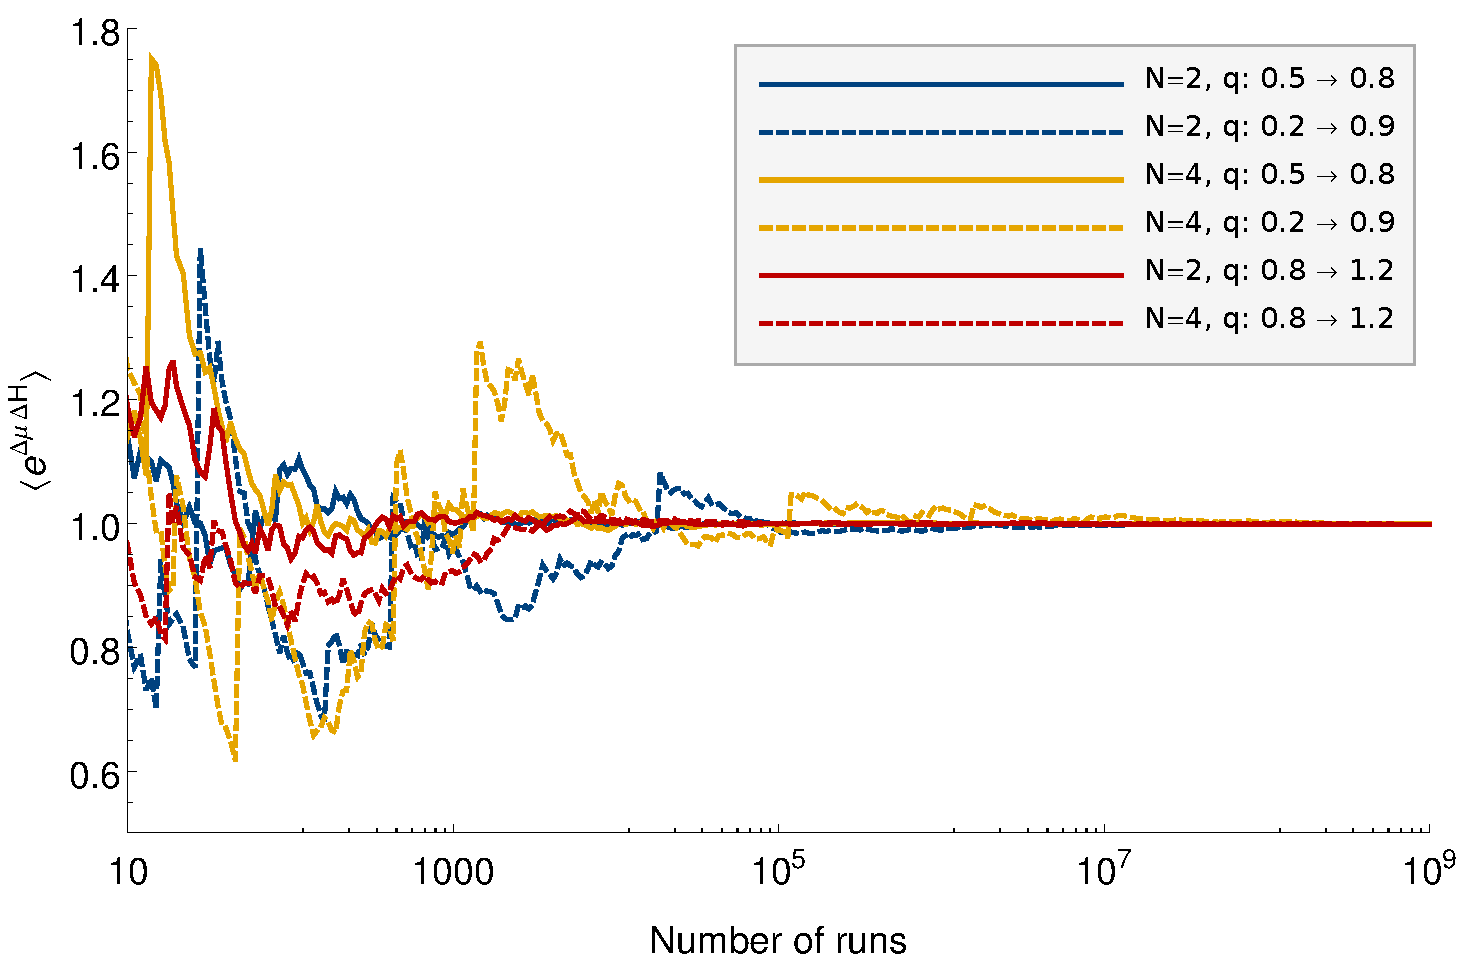
\includegraphics[width=30em]{figures/growth_process}
	\caption[]{Convergence of \(\langle e^{\Delta\mu\Delta H}\rangle\) to~1 in the growth model with system sizes of~{\color{blue}2} and~{\color{dyellow}4}. The initially empty lattice is equilibriated using 50 time steps to reach the initial configuration, before the final state is obtained using three additional steps. Each run records one value \(e^{\Delta\mu\Delta H}\), which is then averaged over many individual runs. The {\color{blue}blue} and {\color{dyellow}yellow} graphs show the development of said average over time in an ordinary quench, and confirm the fluctuation theorem's claim. The {\color{red}red} line corresponds to changing the rates so that the system is brought beyond the phase transition (\(q > 1\)); in this scenario, there is no relaxation into a new stationary state, as the interface grows arbitrarily high over time. Remarkably, the fluctuation theorem seems to hold even in this case, despite the assumption of asymptotic equilibrium in its derivation.}
	\label{fig:growth_process_plot}
\end{figure}




%%%%%%%%%%%%%%%%%%%%%%%%%%%%%%%%%%%%%%%%%%%%%%%%%%%%%%%%%%%%%%%%%%%%%%%%%%%%%%
\subsubsection{Nonequilibrium model on a small state space}
%%%%%%%%%%%%%%%%%%%%%%%%%%%%%%%%%%%%%%%%%%%%%%%%%%%%%%%%%%%%%%%%%%%%%%%%%%%%%%

To test the more general formula \RefEqn{eqn:SEnv fluctuation theorem}, namely
%
\begin{equation*}
	\tilde P(\Delta\SEnv = X) = e^X \tilde P(\Delta\SEnv = -X) ~,
\end{equation*}
%
a less specialized setup is necessary. Here, we will only assume the most basic requirements for this theorem, namely having a Markov process with time-independent rates; more explicitly, there will be no assumptions of equilibirum or asymptotic behaviour.

The system consists of a set of states \(c_i\in\Omega\) with \(|\Omega| = 8\), and therefore a transition matrix \(w_{c\to c'}\) with \(8^2-8 = 56\) nonzero entries (\(\forall c.\;w_{c\to c} = 0\)). Its elements are randomly chosen (strictly) between \(0\) and \(1\) before the experiment (and left fixed throughout each run). In a similar fashion, the initial distribution \(p^\init\) is determined.

A single run now consists of sampling an initial state from \(p^\init\), and letting it evolve in a Monte-Carlo simulation for some time \(T\) (here: \(1\)), corresponding to a certain amount of attempted state transitions (here: \(10^5\)). Each time the system's configuration changes, the generated \(\Delta\SEnv\) is recorded. As an additional consistency check, the overall distriburion of final states was checked against a numerical solution of the Mater equation
%
\begin{equation}
	\forall c.\;\dot p_c(t) = \underbrace{\sum_{c'}w_{c'\to c}p_{c'}(t)}_{\text{jump into } c} - \underbrace{\sum_{c'} w_{c\to c'}p_{c}(t)}_{\text{jump out of } c} ~,
\end{equation}
%
which describes the distribution of states on a statistical level directly, whereas the main simulation is based on individual runs, which are then later used for statistics.


A simulation now consists of a decent amount (\(10^7\)) individual runs, the result of which is then binned and put in a histogram. As can be seein in figures \RefFigure{fig:histogram_lin}~and~\RefFigure{fig:histogram_log}, the theorem is reproducible in simulation.


\begin{figure}[htbp]
	\centering
	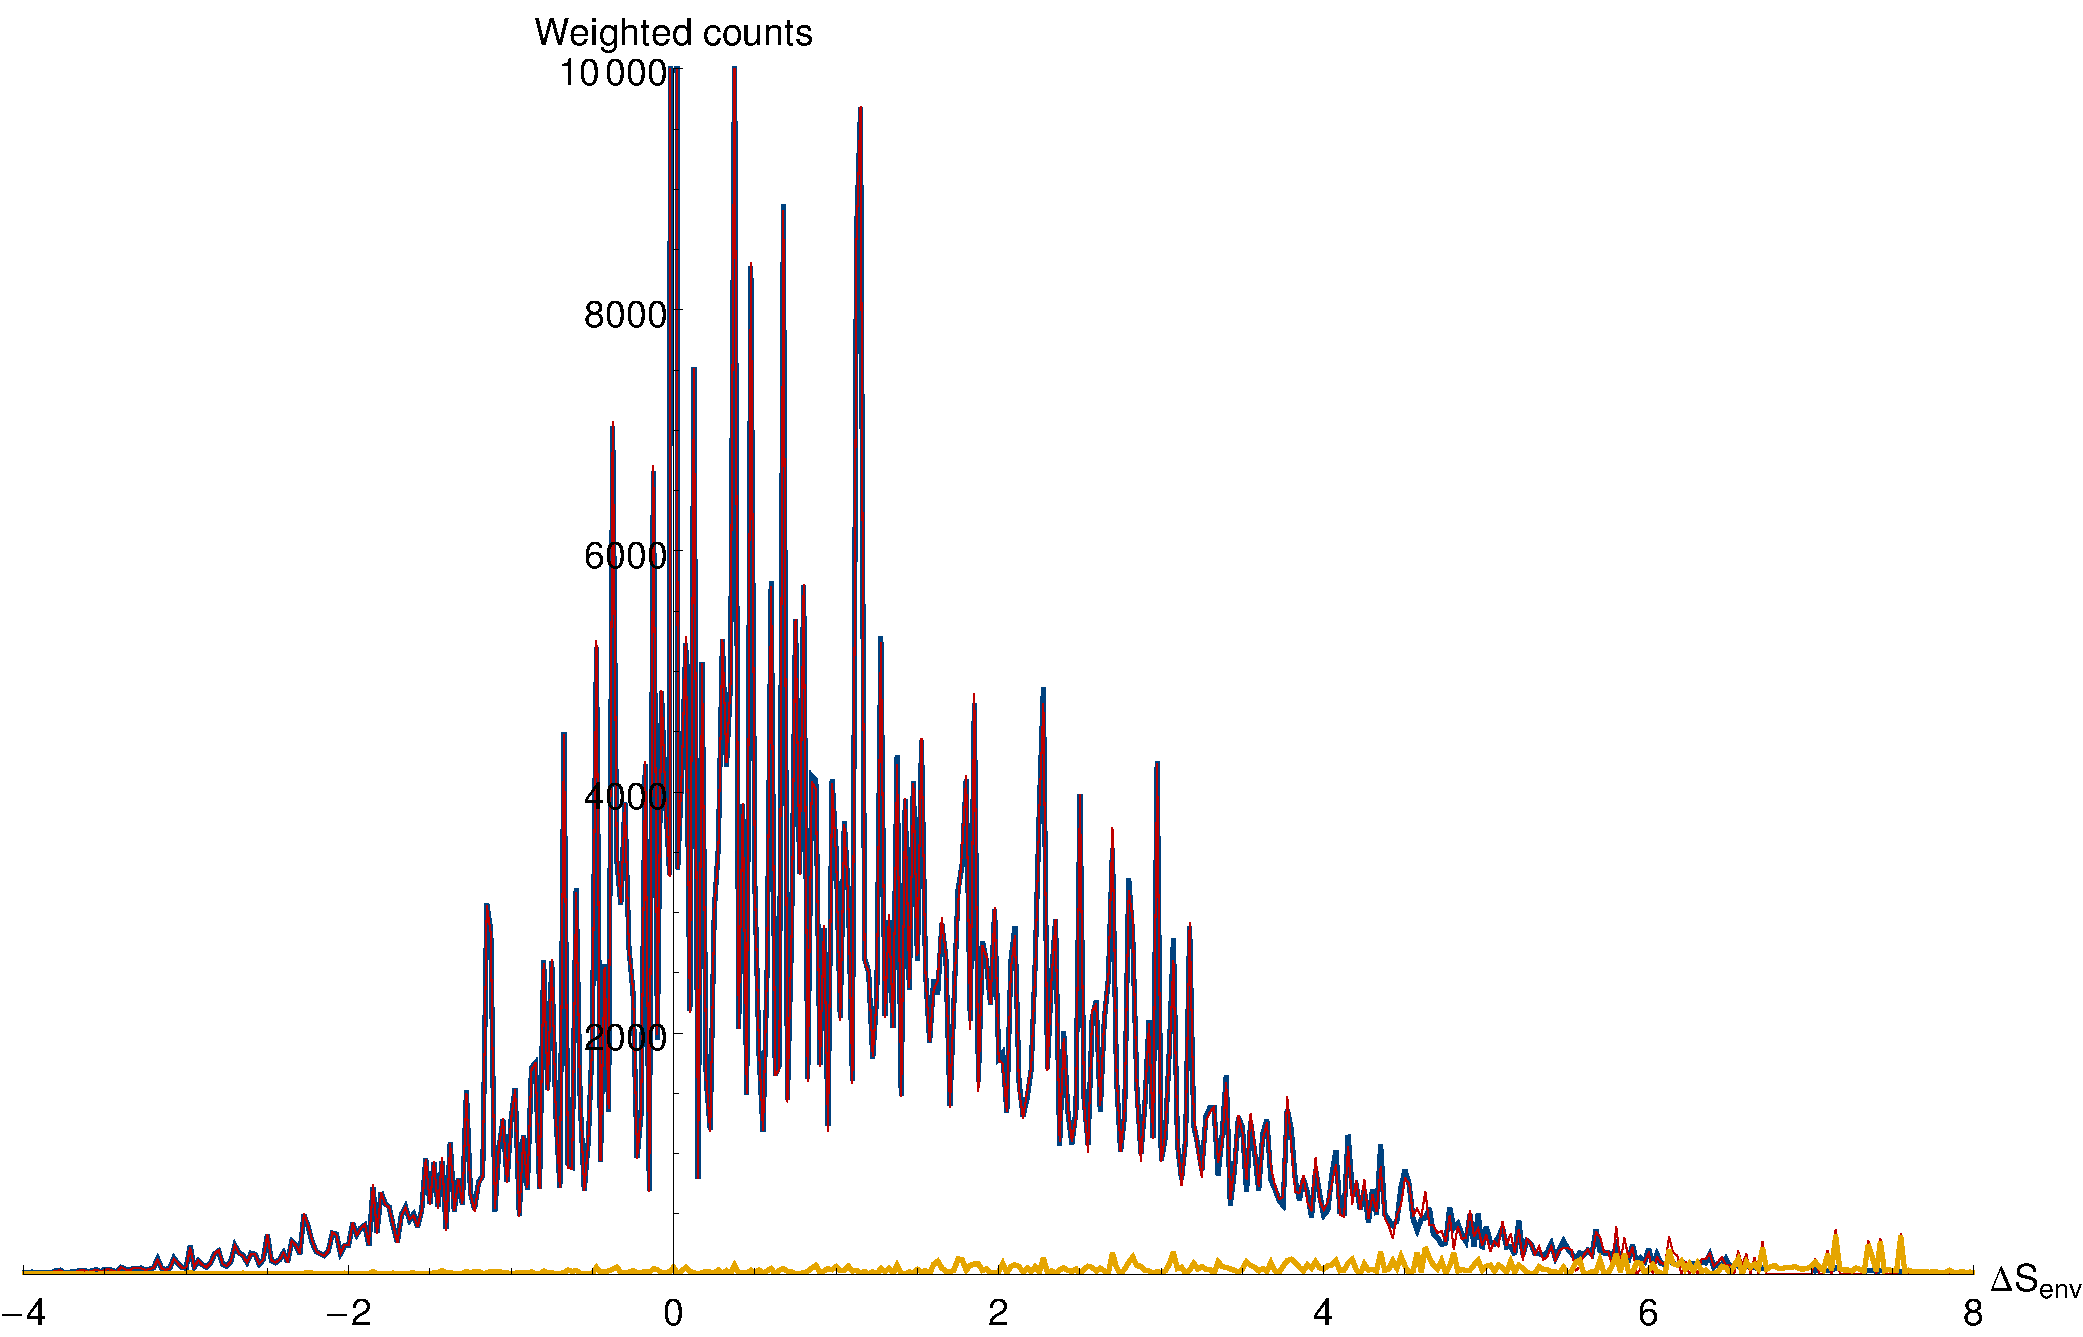
\includegraphics[width=30em]{figures/histogram_lin}
	\caption[]{Linear histogram of a simulation of the fluctuation theorem for \(\Delta\SEnv\), obtained by binning the results of \(10^7\) individual runs. Shown in {\color{blue}blue} and {\color{red}red} are the actual histogram and that histogram with the symmetry relation \(f(x) = e^xf(-x)\) (corresponding to the fluctuation theorem) applied; the {\color{dyellow}yellow} line is the (absolute) deviation between these two representations. It can be seen that both histograms match well, with only a few barely visible red peaks overshooting, which is visualized by the {\color{dyellow}yellow} graph more clearly. The overlap is especially good in the region around \(\Delta\SEnv = 0\) (most notably \emph{at} \(0\), where two peaks about \(5\cdot10^4\) meet), whereas in the large deviation regime towards the edges of the plot show rare events for which the statistics are not as good, but still well within acceptable bounds.}
	\label{fig:histogram_lin}
\end{figure}

\begin{figure}[htbp]
	\centering
	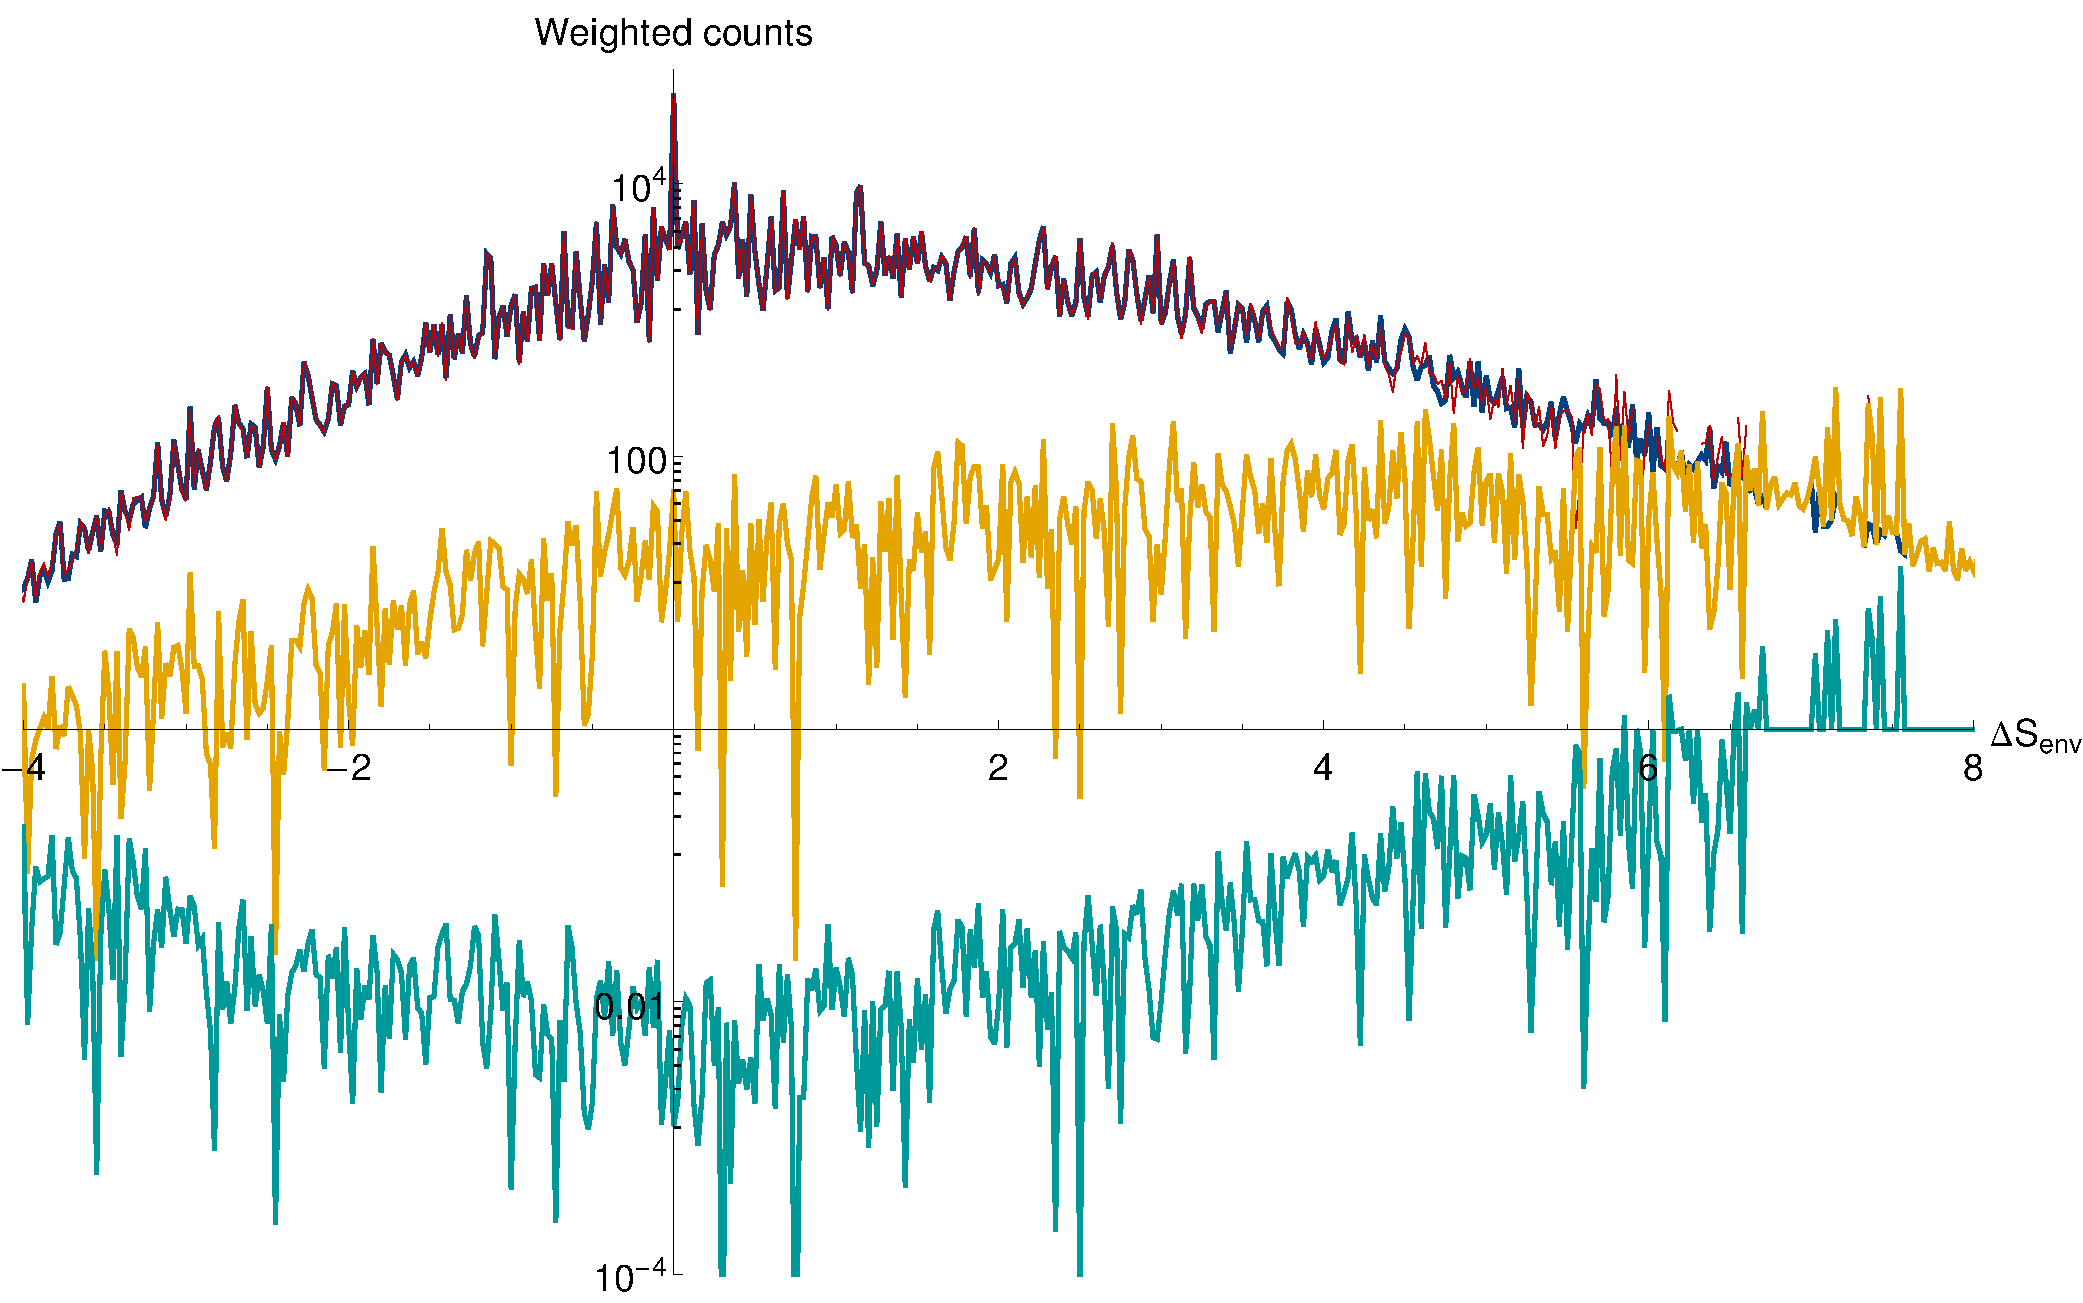
\includegraphics[width=30em]{figures/histogram_log}
	\caption[]{Same histogram as figure \RefFigure{fig:histogram_lin}, but with logarithmic \(y\)-axis. In addition to the graphs for the histogram ({\color{blue}blue}), the symmetrized version ({\color{red}red}, again just barely visible) and the absolute deviation ({\color{yellow}yellow}), this also shows the relative deviation in {\color{cyan}cyan}. This demonstrates again that both graphs match fairly well, particularly in around \(\Delta\SEnv = 0\), where most events happen. Leaving the middle region the overlap becomes worse as \(|\Delta\SEnv|\) increases, which can be explained by the fact that these events are relatively rare, hence the statistics aren't as good (compare e.g. about \(100\) weighted counts at \(\Delta\SEnv = 7\) vs. \(10^4\) around \(\Delta\SEnv = 1\)).}
	\label{fig:histogram_log}
\end{figure}